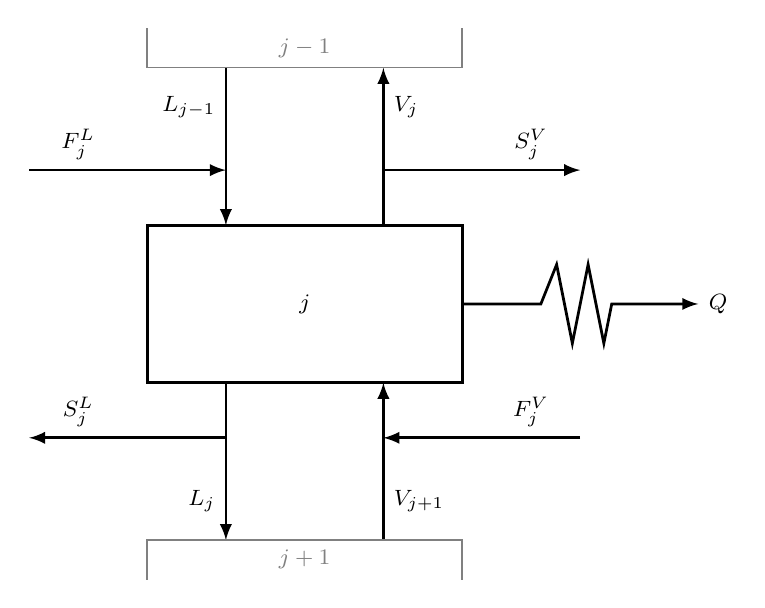
\begin{tikzpicture}[arrow/.style={line width=1pt,->,>=latex}]
	\draw [line width=1pt] (-2,1) rectangle (2,-1) node at (0,0) {\footnotesize $j$};
	\draw [arrow] (-1,3) -- (-1,1) node [pos=0.25, left] {\footnotesize $L_{j-1}$};
 	\draw [arrow] (-3.5,1.7) -- (-1,1.7) node [pos=0.25, above] {\footnotesize $F^L_{j}$};
 	\draw [arrow] (1,1) -- (1,3) node [pos=0.75, right] {\footnotesize $V_{j}$};
 	\draw [arrow] (1,1.7) -- (3.5,1.7) node [pos=0.75, above] {\footnotesize $S^V_{j}$};
 	\draw [arrow] (-1,-1) -- (-1,-3) node [pos=0.75, left] {\footnotesize $L_{j}$};
 	\draw [arrow] (-1,-1.7) -- (-3.5,-1.7) node [pos=0.75, above] {\footnotesize $S^L_{j}$};
	\draw [arrow] (1,-3) -- (1,-1) node [pos=0.25, right] {\footnotesize $V_{j+1}$};
	\draw [arrow] (3.5,-1.7) -- (1,-1.7) node [pos=0.25, above] {\footnotesize $F^V_{j}$};
	\draw [arrow] (2,0) -- (3,0) -- (3.2,0.5) -- (3.4,-0.5) -- (3.6,0.5) -- (3.8,-0.5) -- (3.9,0) -- (5,0,0) node [pos=1, right] {\footnotesize $Q$} ;
    \draw [line width=0.5pt,gray] (-2,-3.5) -- (-2,-3) -- (2,-3) node [pos=0.5, below] {\footnotesize $j+1$} -- (2,-3.5) ; 
    \draw [line width=0.5pt,gray] (-2,3.5) -- (-2,3) -- (2,3) node [pos=0.5, above] {\footnotesize $j-1$} -- (2,3.5) ;
\end{tikzpicture}
